\section{Introduction}
\label{sec:introduction}
Tool learning~\citep{qin2023tool} aims to unleash the power of large language models (LLMs) to effectively interact with various tools (APIs) to accomplish complex tasks. By integrating LLMs with APIs, we can greatly expand their utility and empower them to serve as efficient intermediaries between users and the vast ecosystem of applications. Although open-source LLMs, e.g., LLaMA~\citep{touvron2023llama}, have achieved versatile capabilities through instruction tuning~\citep{alpaca,vicuna2023}, they still lack the sophistication in performing higher-level tasks, such as appropriately interacting with tools (APIs) to fulfill complex human instruction.
This deficiency is because current instruction tuning largely focuses on basic language tasks, with a relative neglect of the tool-use domain.
On the other hand, current state-of-the-art (SOTA) LLMs (e.g., ChatGPT~\citep{openaichatgptblog} and GPT-4~\citep{openai2023gpt4}), which have demonstrated impressive competencies in utilizing tools~\citep{bubeck2023sparks}, are closed-source with their inner mechanisms opaque. This limits the democratization of AI technologies and the scope of community-driven innovation and development.
In this regard, we deem it urgent to \textit{empower open-source LLMs to skillfully master diverse APIs.}
% Besides, such data can be constructed efficiently using self-instruct~\citep{wang2022self}, in a manner similar to performing knowledge distillation from SOTA LLMs.
% show that the capability gap between open-source LLMs and SOTA LLMs can be narrowed by supervised fine-tuning (SFT) on high-quality
% 跟真实场景很接近,不是局限于某一类问题,可落地/可行方案

% After supervised fine-tuning on \ourdata, LLaMA achieves comparable performance compared with \turbo.

\begin{figure*}[!t]
    \centering
    \subfigure{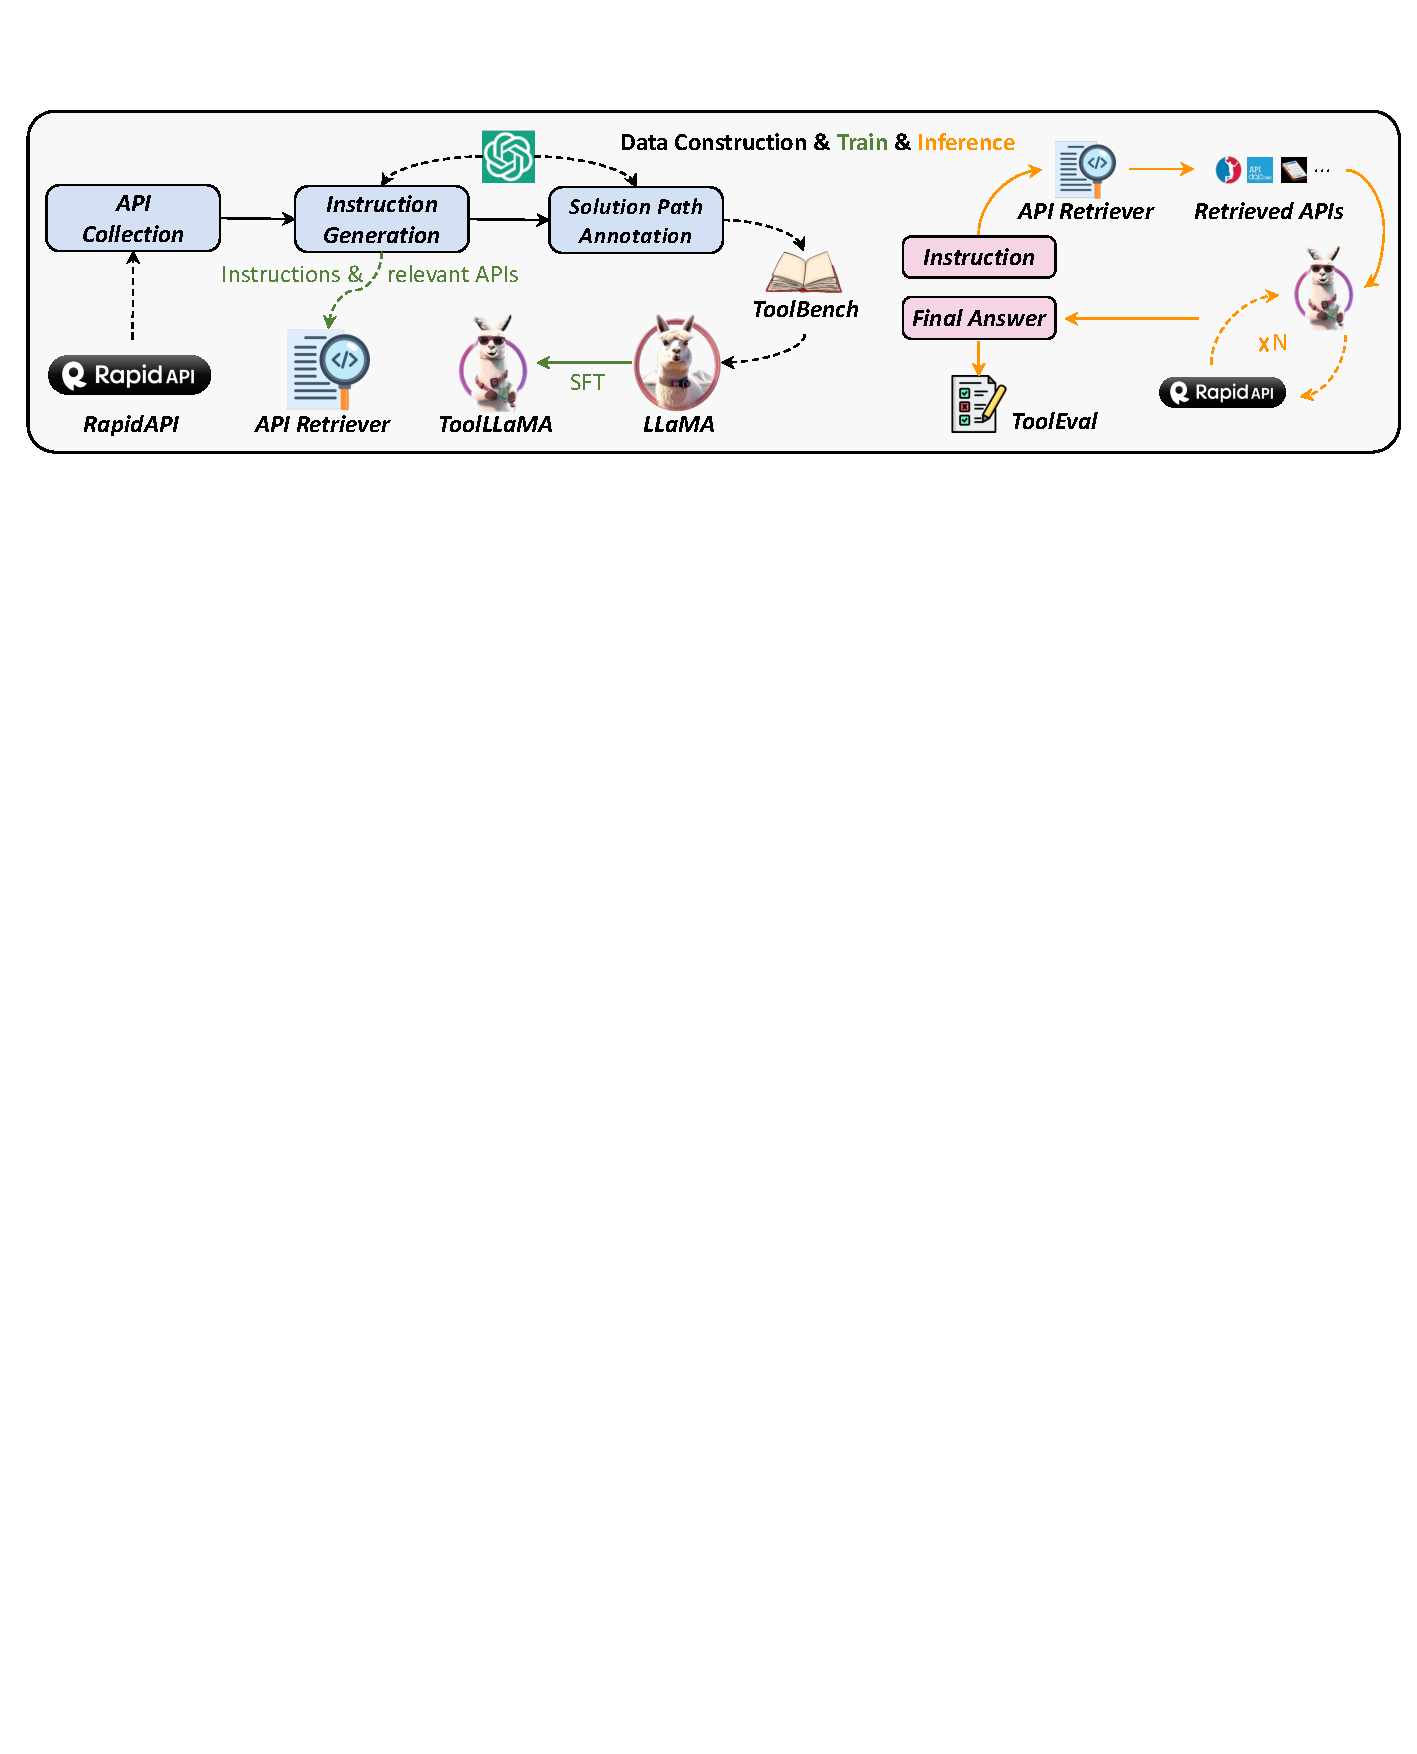
\includegraphics[width=\textwidth]{figs/overview.pdf}}
    \caption{
    \small{Three phases of constructing \ourdata and how we train our API retriever and \ourmodel. During inference of an instruction, the API retriever recommends relevant APIs to \ourmodel, which performs multiple rounds of API calls to derive the final answer. The whole reasoning process is evaluated by ToolEval.
    }
    }
    \label{fig:overview}
\end{figure*}

Although prior works have explored building instruction tuning data for tool use~\citep{li2023api,patil2023gorilla,tang2023toolalpaca,xu2023tool}, they fail to fully stimulate the tool-use capabilities within LLMs and have inherent limitations: (1) \textbf{limited APIs}: they either fail to involve real-world APIs (e.g., RESTAPI)~\citep{patil2023gorilla,tang2023toolalpaca} or consider only a small scope of APIs with poor diversity~\citep{patil2023gorilla,xu2023tool,li2023api};
\begin{wrapfigure}{r}{0.4\textwidth}
  \begin{center}
    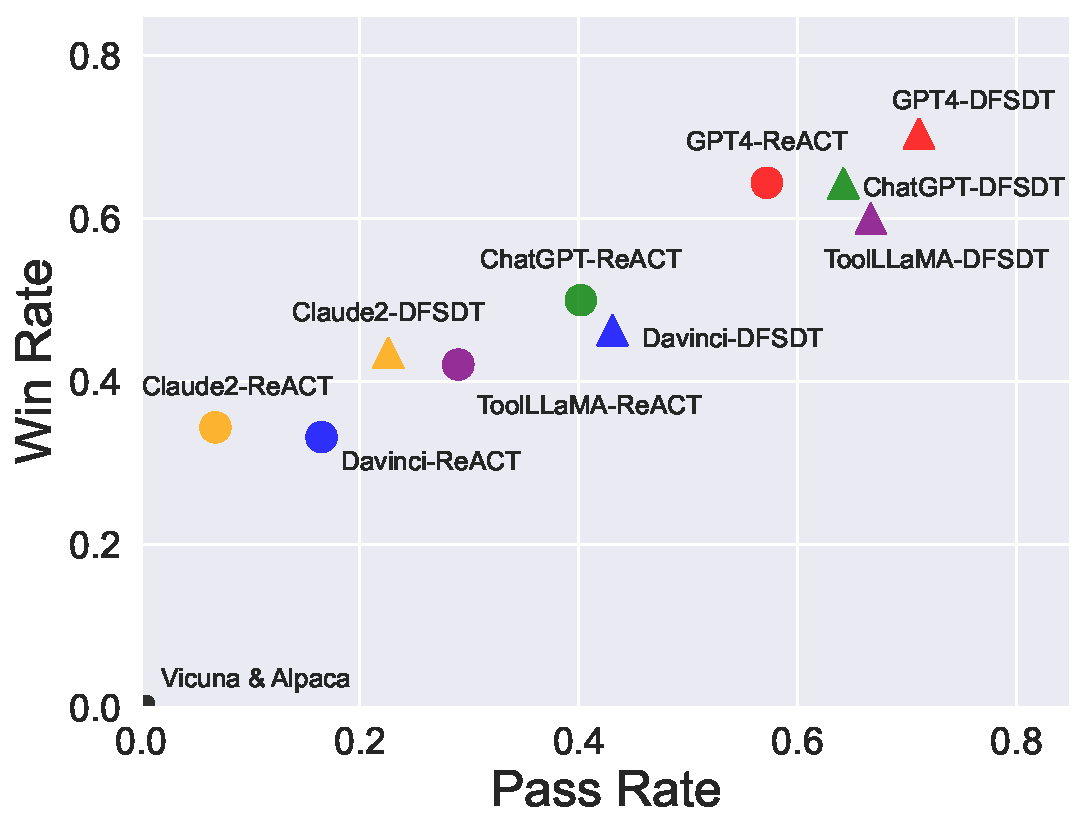
\includegraphics[width=\linewidth]{figs/toolllama_scatterplot.pdf}
  \end{center}
  \caption{
    \small{Pass rate ($\uparrow$) and win rate ($\uparrow$) of different methods in tool-use evaluation. For win rate, we compare each method with ChatGPT-ReACT. \dfs is our improved reasoning strategy over ReACT. \ourmodel surpasses Text-Davinci-003, Claude-2, and almost performs on par with ChatGPT.}
    }
    \label{fig:show_figure}
\end{wrapfigure}
(2) \textbf{constrained scenario}: existing works are confined to instructions that only involve one single tool. In contrast, real-world scenarios may require that multiple tools are interleaved together for multi-round tool execution to solve a complex task. Besides, they often assume that users manually specify the ideal API set for a given instruction in advance, which is infeasible with a large collection of real-world APIs; (3) \textbf{inferior planning and reasoning}: existing works adopted either CoT~\citep{wei2023chainofthought} or ReACT~\citep{yao2022react} for model reasoning, which cannot fully elicit the capabilities stored in LLMs and thus fail to handle complex instructions. 
In addition, some works do not even execute APIs to obtain real responses~\citep{patil2023gorilla,tang2023toolalpaca}, which serve as important information for subsequent model planning.
% This issue is particularly severe for open-source LLMs, which exhibit markedly inferior reasoning ability compared with their SOTA counterparts.

To facilitate tool-use capabilities within open-source LLMs, we introduce \textbf{ToolLLM}, a general tool-use framework including data construction, model training, and evaluation.
As illustrated in Figure~\ref{fig:overview}, we collect a high-quality instruction-tuning dataset \textbf{\ourdata}. It is constructed automatically using ChatGPT (\textit{gpt-3.5-turbo-16k}), which has been upgraded with function call (\textcolor{blue}{\href{https://openai.com/blog/function-calling-and-other-api-updates}{link}}) capabilities. The comparison between \ourdata and prior works is listed in Table~\ref{tab:dataset_comparison}.
Specifically, the construction of \ourdata entails three phases: 


\begin{itemize} [topsep=1pt, partopsep=1pt, leftmargin=12pt, itemsep=-1pt]
    \item \textbf{API Collection}: we gather $\textbf{16,464}$ representational state transfer (REST) APIs from RapidAPI (\textcolor{blue}{\href{https://rapidapi.com/hub}{link}}), a platform that hosts massive real-world APIs provided by developers. 
    These APIs span $\mathbf{49}$ diverse categories such as social media, e-commerce, and weather. For each API, we crawl detailed API documents from RapidAPI, including the functionality descriptions, required parameters, code snippets for API calls, etc. By comprehending these documents to learn to execute APIs, LLMs can generalize to new APIs unseen during training;

    \item \textbf{Instruction Generation}: we first sample APIs from the whole set and then prompt ChatGPT to generate diverse instructions for these APIs. To cover practical scenarios, we curate instructions that involve both \textbf{single-tool} and \textbf{multi-tool} scenarios. This ensures that our model learns not only how to interact with individual tools but also how to combine them to accomplish complex tasks;

    \item \textbf{Solution Path Annotation}: %we annotate high-quality solution paths to these instructions. 
    each solution path may contain multiple rounds of model reasoning and real-time API calls to derive the final response.
    However, even the most sophisticated LLM, i.e., GPT-4, achieves a low pass rate for complex human instructions, making annotation inefficient. To this end, we develop a novel \textbf{depth-first search-based decision tree} (\dfs) to bolster the planning and reasoning ability of LLMs. Compared with conventional ReACT, \dfs enables LLMs to evaluate a multitude of reasoning paths and make deliberate decisions to either retract steps or proceed along a promising path. In experiments, \dfs significantly improves the annotation efficiency and successfully completes those complex instructions that cannot be fulfilled using ReACT.
\end{itemize}

\begin{table*}[!t]
    \centering
    \small
    \resizebox{0.95\linewidth}{!}{
    \begin{tabular}{lccccc}
        \toprule
        \textbf{Resource} & \makecell{\textbf{\ourdata}\\(this work)}& \makecell{ \textbf{APIBench} \\\citep{patil2023gorilla} } & 
        \makecell{ \textbf{API-Bank}\\\citep{li2023api} } &  \makecell{ \textbf{ToolAlpaca} \\\citep{tang2023toolalpaca} } & \makecell{ \textbf{ToolBench}\\\citep{xu2023tool} } 
        \\
         \cmidrule(lr){1-1}  \cmidrule(lr){2-2}  \cmidrule(lr){3-3}  \cmidrule(lr){4-4}  \cmidrule(lr){5-5} \cmidrule(lr){6-6}
          Real-world API?   & \cmark & \xmark & \cmark & \xmark & \cmark  \\ 
          Real API Call\&Response? & \cmark & \xmark & \cmark & \xmark & \cmark  \\ 
          Multi-tool Scenario?   & \cmark & \xmark & \xmark & \xmark & \xmark  \\ 
          API Retrieval?   & \cmark & \cmark & \xmark & \xmark & \cmark  \\ 
          Multi-step Reasoning?   & \cmark & \xmark & \cmark & \cmark & \cmark  \\ 
          \hdashline
          Number of tools   & $\mathbf{3451}$ & $3$ & $53$ & $400$ & $8$ \\ 
          Number of APIs   & $\mathbf{16464}$ & $1645$ & $53$ & $400$ & $232$ \\ 
          Number of Instances   & $\mathbf{126486}$ & $17002$ & $274$ & $3938$ & $2746$ \\ 
          Number of Real API Calls   & $\mathbf{469585}$ & $0$ & $568$ & $0$ & $3926$ \\ 
          Avg. Reasoning Traces  & $4.0$ & $1.0$ & $2.1$ & $1.0$ & $\mathbf{5.9}$ \\ 
         \bottomrule
    \end{tabular}
    }
    \caption{
    \small{A comparison of our \ourdata to notable instruction tuning dataset for tool learning.
    }
    }
    \label{tab:dataset_comparison}
\end{table*}

To assess the tool-use capabilities of LLMs, we develop an automatic evaluator, \textbf{ToolEval}, backed up by \turbo. It comprises two key metrics: (1) \textit{pass rate}, which measures LLM's ability to successfully execute an instruction within limited budgets, and (2) \textit{win rate}, which compares the quality and usefulness of two solution paths. We demonstrate that ToolEval achieves a high correlation with human evaluation and provides a robust, scalable, and reliable assessment for machine tool use.

By fine-tuning LLaMA on \ourdata, we obtain \textbf{\ourmodel}. After evaluation based on our ToolEval, we derive the following findings:

\begin{itemize} [topsep=1pt, partopsep=1pt, leftmargin=12pt, itemsep=-1pt]
    \item \ourmodel demonstrates a compelling capability to handle both single-tool and complex multi-tool instructions. As depicted in Figure~\ref{fig:show_figure}, \ourmodel outperforms Text-Davinci-003 and Claude-2, achieves comparable performance to the ``teacher model'' \turbo, and is only slightly inferior to GPT4.
    Besides, \ourmodel exhibits \textbf{robust generalization to previously unseen APIs}, requiring only the API documentation to adapt to new APIs effectively. This flexibility allows users to incorporate novel APIs seamlessly, thus enhancing the model's practical utility.

    \item We show that our \dfs serves as a general decision-making strategy to enhance the reasoning capabilities of LLMs. \dfs broadens the search space by considering multiple reasoning traces and achieves significantly better performance than ReACT.

    \item We train a neural \textbf{API retriever}, which alleviates the need for manual selection from the large API pool in practice. As shown in Figure~\ref{fig:overview}, given an instruction, the API retriever recommends a set of relevant APIs, which are sent to \ourmodel for multi-round decision making to derive the final answer.
    Despite sifting through a large pool of APIs, the retriever exhibits remarkable retrieval precision, returning APIs closely aligned with the ground truth.

    \item \ourmodel exhibits strong \textbf{generalization} performance on an \textbf{out-of-distribution} (OOD) dataset APIBench~\citep{patil2023gorilla}. Despite not training on any of the APIs or instructions on APIBench, \ourmodel performs on par with Gorilla, a pipeline specifically designed for APIBench.
\end{itemize}

% In summary, this work targets empowering open-source LLMs to execute complex instructions involving diverse APIs in practical scenarios. We hope this work will inspire further research in the intersection of instruction tuning and tool use.